\documentclass[11pt, oneside]{article}   	
\usepackage{hyperref} 
\usepackage{graphicx}

      		
\usepackage[parfill]{parskip}    		
\usepackage{graphicx}			
									
\usepackage{amssymb}


\title{The User Manual for Git}
\author{Pengfei Meng}
\date{}							

\begin{document}
\maketitle
\section{what is Git}
Git is a free and open source version control system.Version control is the management of changes of documents, computer programs, large websites, and other collections of information. Briefly, we as programers track our code changes, we basically save a initial version if code on git. And when we update codes, we can save it on git again, again, and again. And throughout time as our code continues to change we can look back at all of the changes we have made overtime.
\section{Install GIt}
The first thing that you should do is to install Git. You can download Git on the following website:
\href{https://git-scm.com/book/en/v2/Getting-Started-Installing-Git}{https://git-scm.com/book/en/v2/Getting-Started-Installing-Git}\\
Because I use Mac, so I will mainly introduce how to use git on Mac,and note that for this manual we will be using git on the command line only(Mac's terminal).
\section{The working mechanism of Git}
Using Git, It's essential to know how do Git works. Actually the design of git is very easy and logical, I will show a picture that reveals the basic logic of git for u.\\
\centerline{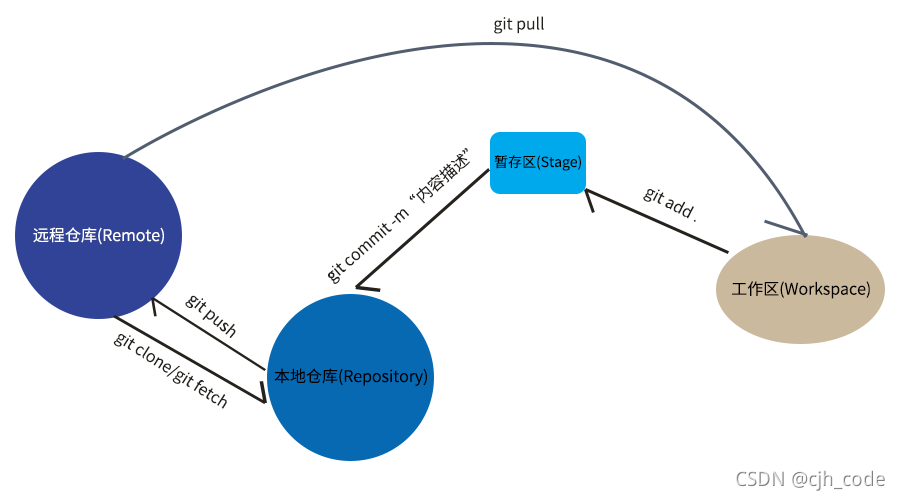
\includegraphics[scale=0.6]{git design.png}}\\
To understand this picture, we need to know some terms firstly:\\

Directory: which is also known as folder on you computer, contains Workspace and Stage.\\
Workspace: where you do coding job.\\
Stage: which saves completed works that are waiting for ``git commit'' 
Repository: Project, or the folder(place) where you project is kept.\\
Github(Remote): A website to host your repository online.you can register a free account in this website:
\href{https://github.com}{https://github.com}

And some Linux commands:\\

git clone: Bring a repository that is hosted somewhere like Github into a folder on your local machine.\\
add: track your changes and files in git.\\
commit: save your files in git.\\
push: upload Git commits to  remote repo, like Github.\\
pull: the opposite of push, download some changes from remote repo to your local machine.\\ 

Hence, there are 4 steps to use git:\\

1.Download and set up git on you machine(about how to set up git, maybe I will post a tutorial to introduce).
2.Log in Github and input the SSH key(that you get from set-up step), then verify link on you machine.
3.create a new repository and clone it to your machine.
4.Do the three commands``git add'', ``git commit -m'', and ``git push''.




\end{document}  